\section{UI}\label{UI}
Each group was given the task to contribute to the \knox{} UI in some way. 
A UI committee was created to manage decisions relating to the UI. 
It was decided the frontend be created in the React JavaScript library\cite{Reactjs}, while the backend server be created in Node.js\cite{Nodejs}.
Each group then had to decide themselves what they wanted to create. 


We decided to create a database and server status component. 
This component would be responsible for displaying the status of both the RDF and WordCount APIs and databases. 
Thus, for both, there are a few cases that must be handled:
\begin{itemize}
	\item The backend server did not respond.
	\item The backend server responded, but the database server did not respond.
	\item The backend and database server responded, but the database itself did not respond.
	\item The backend and database server as well as the database itself all responded.
\end{itemize}

On the frontend, a status message is displayed along with a colored circle to indicate the result of the status check:
\begin{itemize}
	\item Yellow while the client is fetching the database status.
	\item Red if either the backend server, database server or database itself does not respond.
	\item Green for both servers and databases responding.
\end{itemize}
If both APIs and databases respond, the average response time is also displayed.
On the frontend, these features were implemented using simple CSS and React JavaScript code where we use the JavaScript Fetch API to access the Node.js backend server.
On the backend server, a timer is set up to ping both the WordCount and RDF APIs every ten minutes.
The most recent ten results are then stored in an array.
When the frontend requests the status of the databases, the backend calculates the average response time using the stored results which it then includes in its response body.
If the latest database server pings failed, the backend server only includes a status code in its response body indicating that the database servers are down.


Figure \ref{dbstatusUI} shows the database status UI assuming a response from both the WordCount server and database, and no response from the RDF server.
\begin{figure}[htb!]
    \centering
    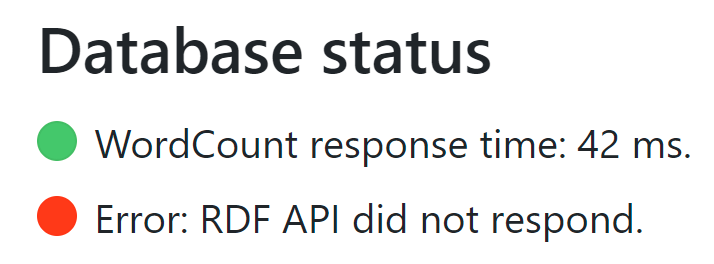
\includegraphics[scale=0.5]{Images/dbstatus.png}
    \caption{The UI indicating the status of the database servers and the databases themselves.}
    \label{dbstatusUI}
\end{figure}
